\section{Discussion} % PRESENT TENSE!!!
\label{sec:discussion}
% TODO: Statistical significance analysis of results and discussion of application of findings.
% % bulletpoint list in latex
% \begin{itemize}
%     \item implications
%     \item threats to validity
%     \item future work
% \end{itemize}

\subsection{Implications}
Our results show that the choice of activation functions remains irrelevant even at smaller scales. All the comparisons in section \ref{sec:results} show that the differences are not statistically significant. This suggests that the choice of activation function does not have a significant impact on the performance of language models with 10 million parameters. This is in contrast to the findings of Mirzadeh et al. \cite{Mirzadeh2023}, who suggested that the impact of activation functions diminishes as the model size increases. Our results suggest that the impact of activation functions is negligible even at smaller scales. Furthermore, the training durations of models employing various activation functions showed minimal differences, indicating that the selection of one activation function over another does not significantly impact training efficiency.\\ 
The comparison of results between GELU and the novel Learnable GELU further corroborates the findings of \textit{Dror et al.} \cite{dror2018hitchhikers}, which emphasize the importance of statistical significance analysis in evaluating various architectural decisions in language models. Our initial findings indicated an improved performance of Learnable GELU, but subsequent analysis revealed these improvements to be statistically insignificant.\\
\\\\
\textbf{ToDo: Add more specific implications of other comparisons.}
\\\\
Models with KAN-Networks do seem to perform better than models with traditional MLPs, as shown by the highest scores achieved by the BERT-KAN and GPT-KAN models. This suggests that the KAN architecture could be beneficial for language models, even at smaller scales. However, the increased number of trainable parameters and increased training times is a significant drawback that needs to be considered. 

\subsection{Threats to validity}
Internal validity examines the certainty that the observed results are due to independent variables and not other factors. External validity concerns the extent to which the findings of the study can be generalized to contexts outside the study. Construct validity refers to the extent to which the measurement tools are appropriate for the study. 

% Limited compute
% only one epoch
% only two different types of models
% we did multiple seeds
\subsubsection{Internal validity}
To ensure that our results were not due to chance, we trained models using six different random seeds. While this sample size is relatively small, it was a necessary compromise given our resource constraints. To address this limitation, we employed bootstrapping with 10,000 samples to calculate confidence intervals and mean differences between models. Additionally, to verify that our findings were not model-specific, we utilized two distinct types of models: an encoder (roBERTa) and a decoder (GPT-Neo). Nevertheless, it is important to note that all models were trained on the same dataset, which may have introduced some bias. The train times could have been affected by busy delft blue nodes, but across models trained on multiple seeds, the training times were relatively consistent with a standard deviation of only 9 minutes and 52 seconds across all models including the ones with KAN - Network. \\ 
Another potential threat to validity is that the implementation of adaptable activation functions added 2048 learnable parameters to each model, which could have influenced the results. However, given that 2048 parameters constitute a relatively small proportion in models with 9M, and the results were not statistically significant, this impact is likely minimal.

% Tiny stories might not be representative 
% Would be trained on more epochs so models would further converge 
% Kan is new, implementation was not perfect, training was unstable
\subsubsection{External validity}
All the models were trained for only one epoch due to computational constraints, resulting in none of the models fully converging. This may have impacted the performance of the models and the significance of the results, as differences might be more pronounced or minimized with additional epochs. In a real-world scenario, models would typically be trained for more epochs. Additionally, the models utilized in this study are not the latest state-of-the-art, which may affect the generalizability of the results. Furthermore, the TinyStories dataset used for pre-training, which comprises only short fictional stories, may not be representative of the datasets typically used for production-level language models.
\textbf{ToDO: talk about kan implementation}
\subsubsection{Construct validity}
The evaluation pipeline used in this study, BabyLM, primarily focuses on grammatical tasks, which may not fully capture the comprehensive capabilities of language models. However, considering the scope of this research, the tasks evaluated by the BabyLM evaluation pipeline are suitable. Since BabyLM is specifically designed for the evaluation of smaller language models, it aligns well with our study's focus. Thus, it is an appropriate tool for assessing the impact of activation functions on these models.

\subsection{Future work}
I hope this research will inspire further studies to give activation functions less attention. Before publishing new activation functions, researchers should conduct multiple runs and perform statistical significance tests to ensure the robustness of their findings. \\ 
The KAN architecture is a relatively new concept, and the implementation used in this study may not have been optimal. Although we utilized more efficient and optimized implementation as suggested by the original paper \cite{Liu2024}, the training process was less stable compared to baseline models (see Figure \ref{fig:grad-norm}), and the models did not converge as expected. This instability may have impacted the performance of the \textsc{KAN models}, suggesting that future research should investigate this issue further. Despite its potential, this promising direction concerning activation functions and its interpretability benefits were not fully explored in this study due to time constraints.

\begin{figure}[ht]
    \centering
    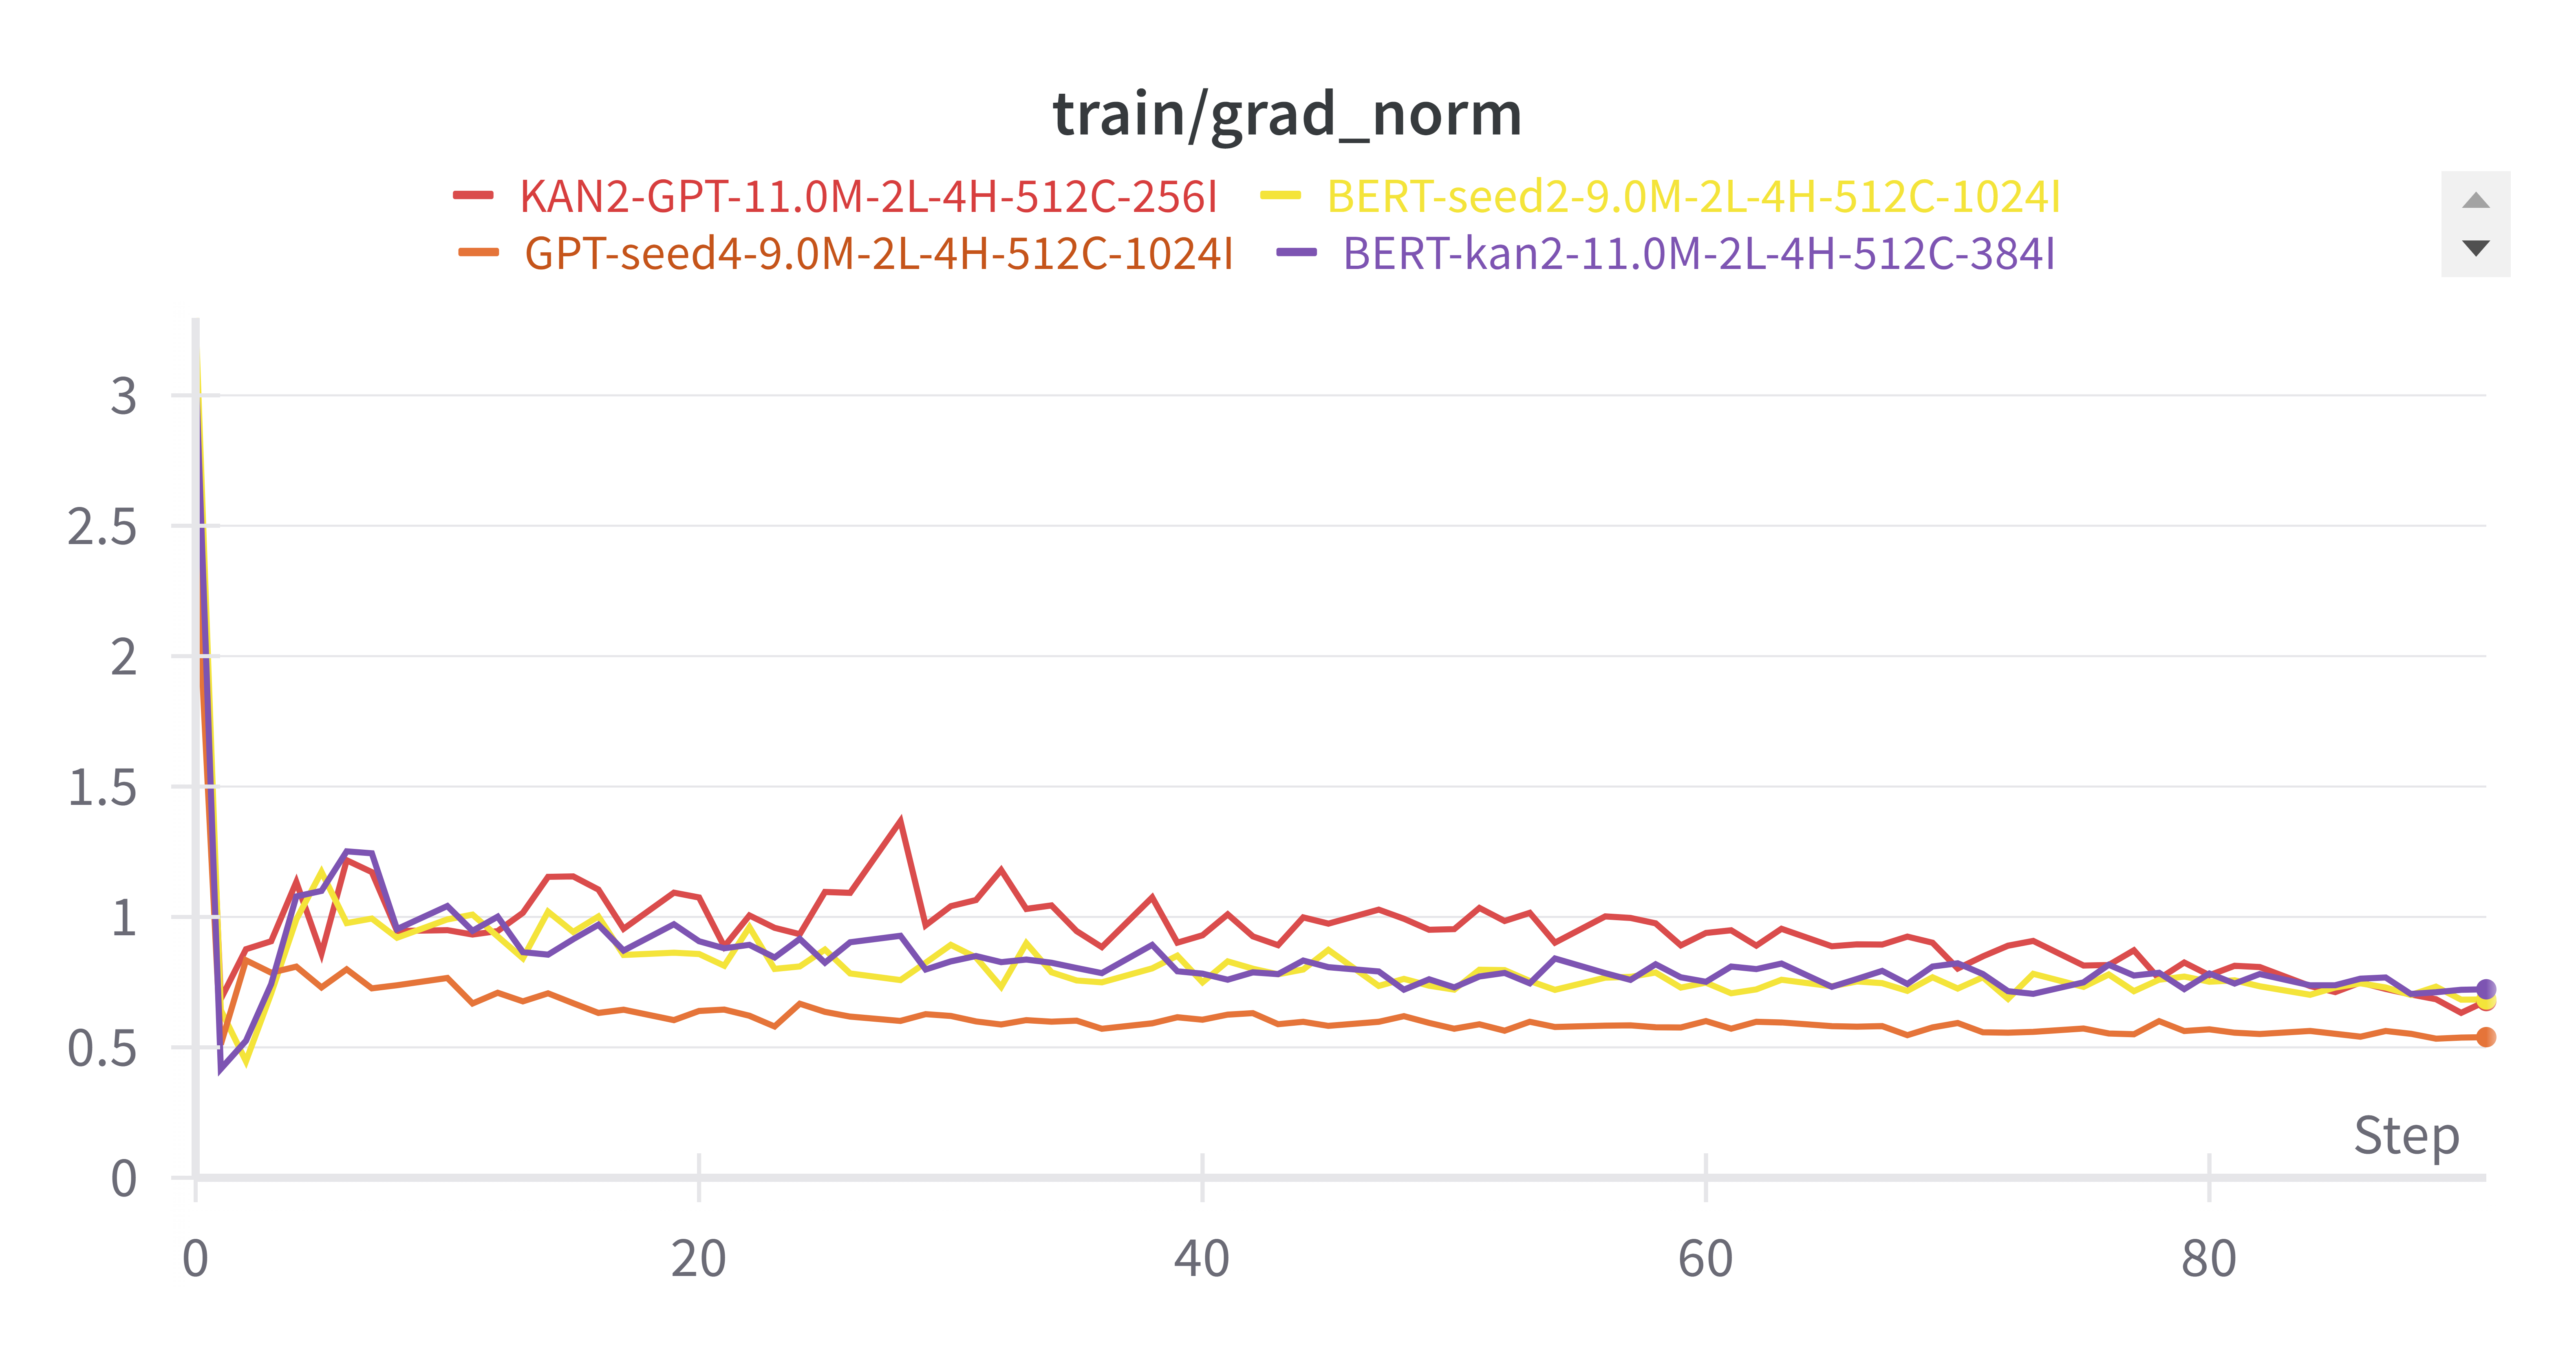
\includegraphics[width=\columnwidth]{figures/train-grad-norm.png}
    \caption{Gradient normalization during training of KAN models. The KAN models show higher variance in gradient norms compared to the baseline models. \textbf{ToDo: Fix readability}}
    \label{fig:grad-norm}
\end{figure}
